\documentclass{article}

\usepackage{graphicx}
\usepackage{amsmath}

\setlength{\parskip}{\medskipamount}

\title{Advanced Object Oriented Programming and Design\\
\medskip
\large Homework 3}
\author{Abraham Murciano and Daniel Klein}

\begin{document}

\maketitle

\section{Eater/Silverware System}

\subsection*{Part A: Basic Design}

Thi system represents Eaters and Silverware. An Eater has an eat operation, and a Silverware has a scoop operation. Each Eater has a single Silverware and he uses its scoop operation. There are two types of Eaters: QuietEater and NoisyEater. There are two types of Silverware: Chopstick and Fork.

\begin{figure}[ht]
	
\includegraphics[width=\textwidth]{hw4q1a.png}
\end{figure}

\subsection*{Part B: Adding a Spoon}

Suppose we are given a compiled Spoon class, having an operation shlook. We would like to use Spoon as an additional Silverware (Where shlook corresponds to scoop). However, we are not allowed to change Spoon's code or even recompile it. Below is a new diagram incorporating Spoon into the system. We used the class adapter pattern.

\begin{figure}[ht]
	
\includegraphics[width=\textwidth]{hw4q1b.png}
\end{figure}

\subsection*{Part C: Adding Drinkers}

We would like to add Drinkers to our system from part A. A Drinker also has a Silverware. In addition, we want to add to each of the existing Silverware a stir operation. Only Drinkers use a Silverware's stir operation and only Eaters use its scoop operation. We must draw a new diagram incorporating Drinkers into the system.

\begin{figure}[ht]
	
\includegraphics[width=\textwidth]{hw4q1c.png}
\end{figure}

\section{Speech Censoring System}

This system represents Mammals. Each Mammal has a speak operation, generating RawData representing the Mammal's voice. A Human is a type of Mammal. Every invocation of speak by a human should be followed by a voice-analysis process. If the Human's voice contains certain words (The list of words may change from one execution to another), the Human will be warned. A Human with 3 warnings executes a function payFine.

Apart from Human, there are additional Mammals (e.g., Dog), but Human is the only Mammal that can be warned. There may be other non-Mammal warn-able classes that generate voice (e.g., Parrot, Gramophone). We must incorporate the following functions.

\begin{description}
	\item[List \(<\text{String}>\) convertSoundToText (RawData voice)] returns a list of words that the voice contains.
	\item[void CensorVoice(RawData voice, ? client)] Analyzes the voice and if it contains certain words, warns the client.
	\item[void warn()] Updates the object that it has been warned.
\end{description}

Below is the design which conforms to the above specification.

\begin{figure}[ht]
	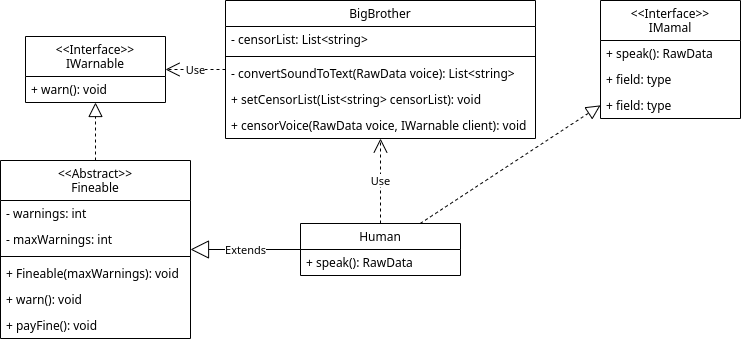
\includegraphics[width=\textwidth]{hw4q2.png}
\end{figure}

\end{document}